\documentclass[tikz,border=10pt]{standalone}
\usetikzlibrary{calc}
\begin{document}
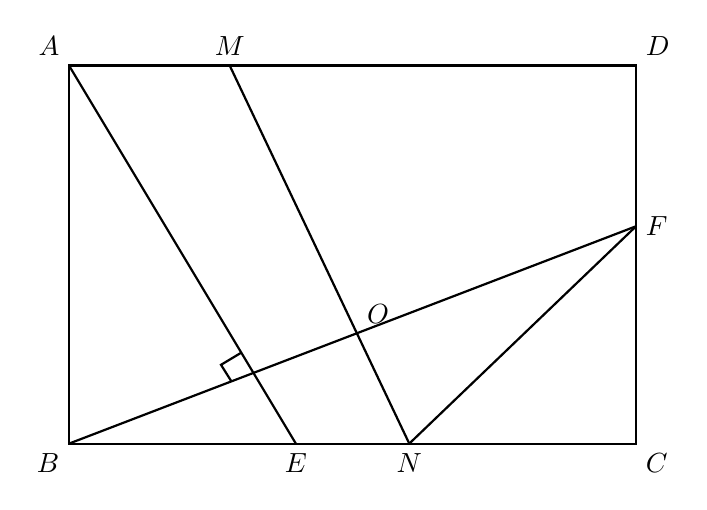
\begin{tikzpicture}[scale=1.2]
\coordinate (A) at (0,4);
\coordinate (B) at (0,0);
\coordinate (C) at (6,0);
\coordinate (D) at (6,4);
\coordinate (M) at (1.7,4);
\coordinate (E) at (2.4,0);
\coordinate (F) at (6,2.3);
\coordinate (N) at (3.6,0);
\coordinate (O) at (3.05,1.167);
\coordinate (P) at (1.951,0.748);

\draw[thick] (A) -- (D) -- (C) -- (B) -- cycle;
\draw[thick] (A) -- (E);
\draw[thick] (M) -- (N);
\draw[thick] (B) -- (F);
\draw[thick] (N) -- (F);

% right angle mark at AE x BF (point P)
\draw[thick] ($(P)!0.25cm!(A)$) -- ($($(P)!0.25cm!(A)$)!0.25cm!90:(A)$) -- ($(P)!0.25cm!(B)$);

\node[above left] at (A) {$A$};
\node[below left] at (B) {$B$};
\node[below right] at (C) {$C$};
\node[above right] at (D) {$D$};
\node[above] at (M) {$M$};
\node[below] at (E) {$E$};
\node[below] at (N) {$N$};
\node[right] at (F) {$F$};
\node[above right] at (O) {$O$};
\end{tikzpicture}
\end{document}
